\section{Diskussion}
\label{sec:Diskussion}
Insgesamt lässt sich fest stellen, dass sowohl die Messung der Massen und Durchmesser der Kugeln als auch die Messung der Fallzeiten ziemlich präzise ist,
da die Messwerte nur geringe Abweichungen haben. Dennoch ist ein systematischer Fehler durch das Stoppen der Uhr nicht auszuschließen. Weiterhin weicht
die Viskosität des Wassers bei Raumtemperatur $\eta_{\symup{RT}}$ um $27\,\%$ vom Literaturwert ab, der bei $1\,\unit{\milli\pascal}\cdot \unit{\second}$
\cite{kritreynold} liegt.\\
Außerdem lässt sich durch die wesentlich kleineren Reynoldszahlen der beiden Kugeln definitv bestätigen, dass es sich im Rohr um laminare und keine turbulenten
Strömungen handelt. Hinzu kommt noch, dass die Messwerte auch alle sehr nah an der Ausgleichsgerade liegen, so dass keine etwaigen Ausreißer betrachtet werden müssen.

\section{Messwerte}
\label{sec:Messwerte}
\begin{figure}[h]
  \centering
  \begin{subfigure}{0.5\textwidth}
    \centering
    \includegraphics[width=0.75\textwidth]{GroßeKugel.jpeg}
    \caption{Messdaten der Radien und Massen der beiden Kugeln.}
  \end{subfigure}

  \begin{subfigure}{0.5\textwidth}
    \centering
    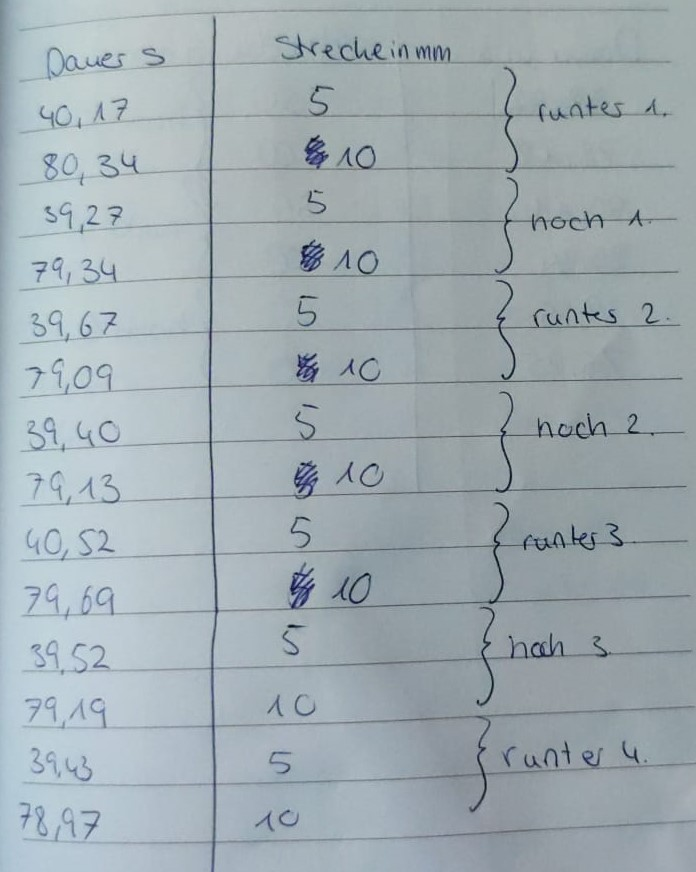
\includegraphics[width=0.75\textwidth]{GrKugel1.jpeg}
    \caption{Fallzeiten der großen Kugel 1.}
  \end{subfigure}

  \begin{subfigure}{0.5\textwidth}
    \centering
    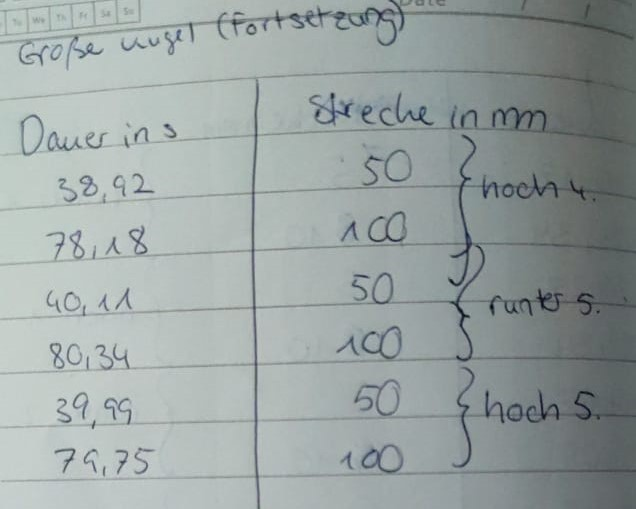
\includegraphics[width=0.75\textwidth]{GrKugel2.jpeg}
    \caption{Fallzeiten der großen Kugel 2.}
  \end{subfigure}
  \caption{Messdaten 1.}
\end{figure}

\begin{figure}
  \centering
  \begin{subfigure}{0.5\textwidth}
    \centering
    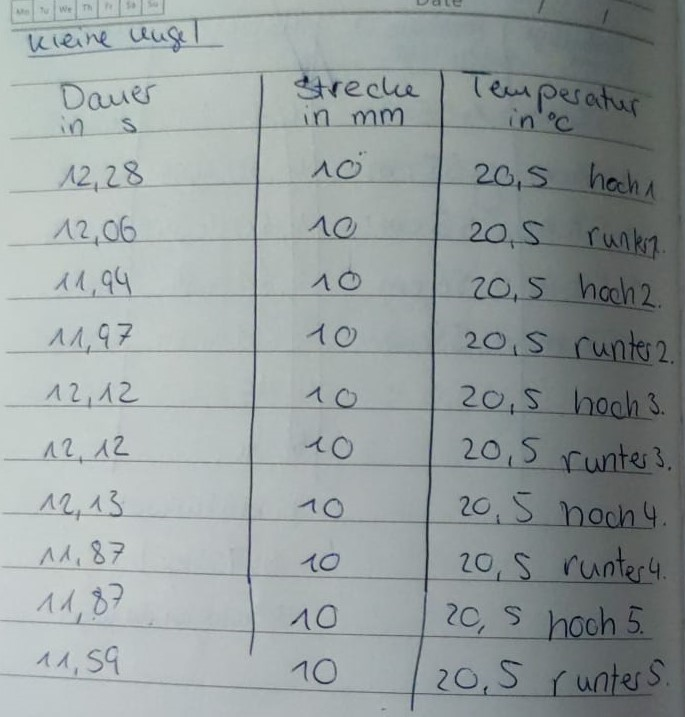
\includegraphics[width=0.75\textwidth]{KleineKugel1.jpeg}
    \caption{Fallzeiten der kleinen Kugel 1.}
  \end{subfigure}

  \begin{subfigure}{0.5\textwidth}
    \centering
    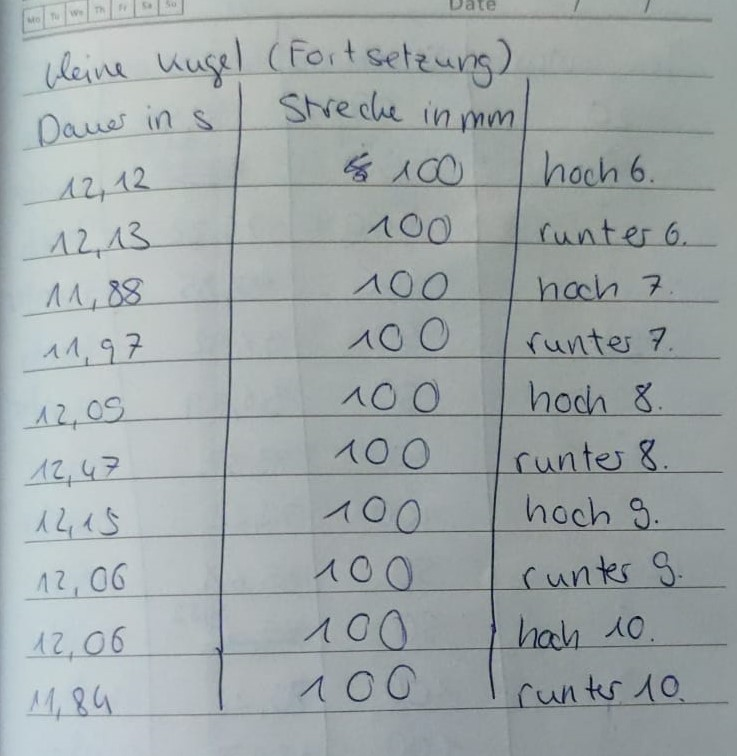
\includegraphics[width=0.75\textwidth]{KleineKugel2.jpeg}
    \caption{Fallzeiten der kleinen Kugel 2.}
  \end{subfigure}

  \begin{subfigure}{0.5\textwidth}
    \centering
    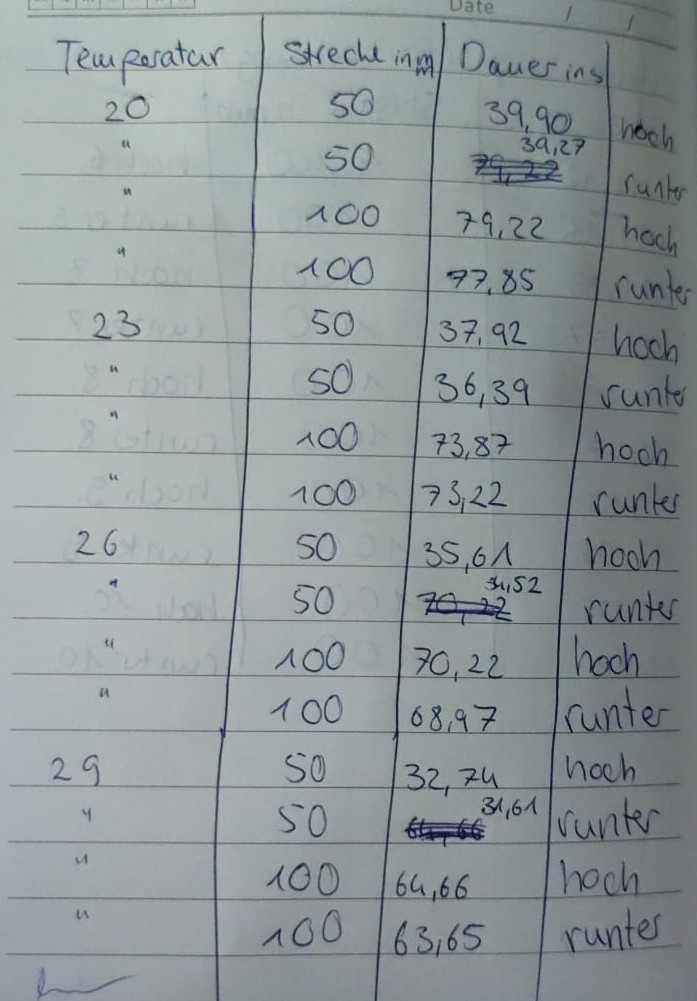
\includegraphics[width=0.75\textwidth]{Temp1.jpeg}
    \caption{Messung der Viskosität in Abhängigkeit der Temperatur 1.}
  \end{subfigure}
  \caption{Messdaten 2.}
\end{figure}

\begin{figure}
  \centering
  \begin{subfigure}{0.5\textwidth}
    \centering
    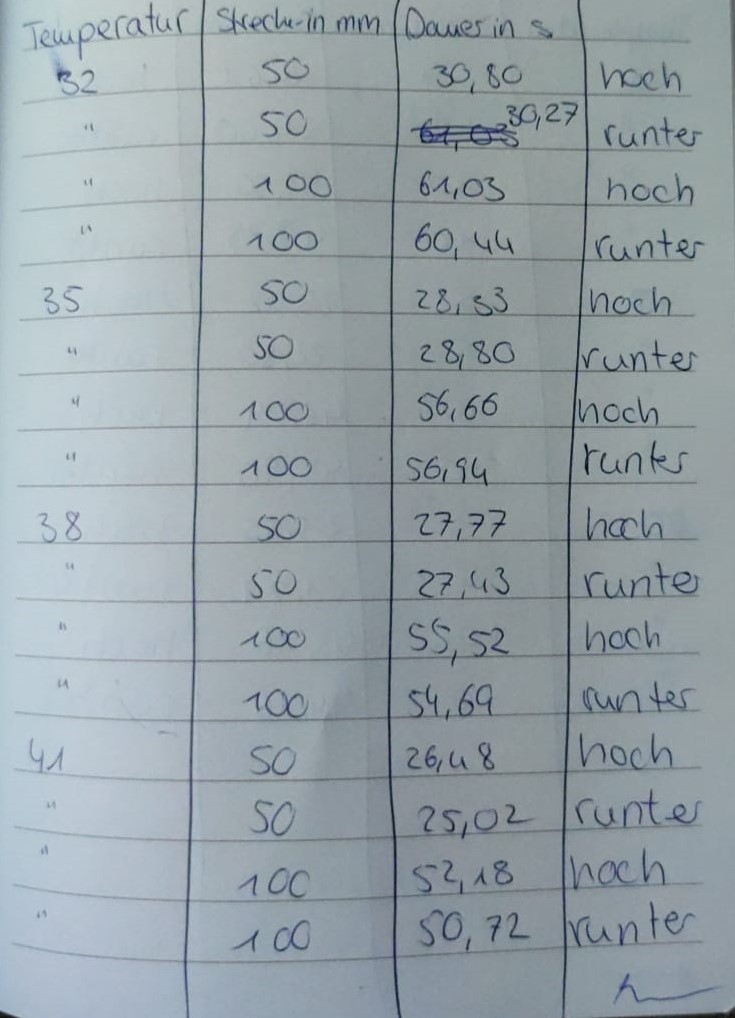
\includegraphics[width=0.75\textwidth]{Temp2.jpeg}
    \caption{Messung der Viskosität in Abhängigkeit der Temperatur 2.}
  \end{subfigure}

  \begin{subfigure}{0.5\textwidth}
    \centering
    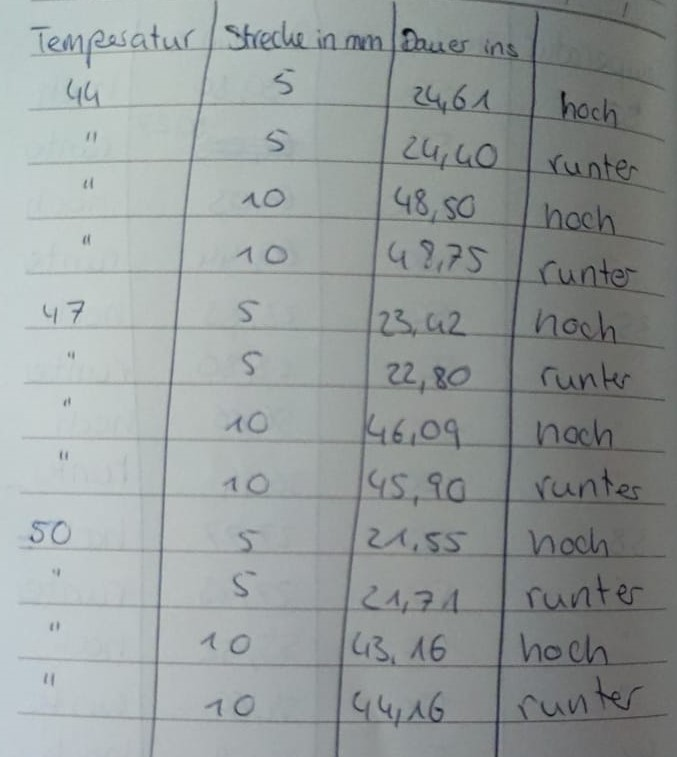
\includegraphics[width=0.75\textwidth]{Temp3.jpeg}
    \caption{Messung der Viskosität in Abhängigkeit der Temperatur 3.}
  \end{subfigure}
  \caption{Messdaten 3.}
\end{figure}